\chapter{磁  场}

\section{磁场 安培力}

1.磁场、磁感应强度

(1)磁场的基本性质

磁场对处于其中的磁体、电流和运动电荷有\_\_磁力\_\_的作用.

(2)磁感应强度

\ding{172}物理意义:描述磁场的\_\_强弱和方向\_\_.

\ding{173}定义式:$B=\dfrac{F}{I L}$(通电导线垂直于磁场).

\ding{174}方向:小磁针静止时 N极的指向 .

\ding{175}单位:\_\_特斯拉\_\_,符号T.

(3)匀强磁场

\ding{172}定义:磁感应强度的大小\_\_处处相等\_\_、方向\_\_处处相同\_\_的磁场称为匀强磁场.

\ding{173}特点:疏密程度相同、方向相同的平行直线.

(4)地磁场

\ding{172}地磁的N极在地理\_\_南极\_\_附近,S极在地理\_\_北极\_\_附近,磁感线分布如图所示.

\begin{center}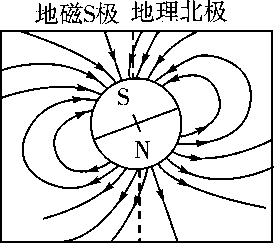
\includegraphics[width=1.24514in,height=1.10347in]{media/image335.png}\end{center}

\ding{173}在赤道平面上,距离地球表面高度相等的各点,磁感应强度\_\_大小相等\_\_,且方向水平\_\_向北\_\_.
\newpage
2.磁感线和电流周围的磁场

(1)磁感线的特点

\ding{172}磁感线上某点的\_\_切线方向\_\_就是该点的磁场方向.

\ding{173}磁感线的疏密程度定性地表示磁场的\_\_强弱\_\_,在磁感线较密的地方磁场\_\_较强\_\_;在磁感线较疏的地方磁场\_\_较弱\_\_.

\ding{174}磁感线是闭合曲线,没有起点和终点.在磁体外部,从\_\_N极\_\_指向\_\_S极\_\_,在磁体内部,由\_\_S极\_\_指向\_\_N极\_\_.

\ding{175}同一磁场的磁感线不\_\_中断\_\_、不\_\_相交\_\_、不相切.

⑤磁感线是假想的曲线,客观上不存在.

(2)电流周围的磁场(安培定则)

\begin{longtable}[]{@{}m{2cm}m{3cm}m{3cm}m{3cm}@{}}
\toprule
 & \begin{minipage}[b]{0.22\columnwidth}\raggedright
直线电流的磁场\strut
\end{minipage} & \begin{minipage}[b]{0.22\columnwidth}\raggedright
通电螺线管的磁场\strut
\end{minipage} & \begin{minipage}[b]{0.22\columnwidth}\raggedright
环形电流的磁场\strut
\end{minipage}\tabularnewline
\midrule
\endhead
特点 & 无磁极、非匀强磁场且距导线越远处磁场越弱 &
与条形磁铁的磁场相似,管内为匀强磁场且磁场最强,管外为非匀强磁场 &
环形电流的两侧是N极和S极且离圆环中心越远,磁场越弱\tabularnewline
安培定则 &
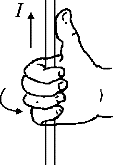
\includegraphics[width=0.54722in,height=0.75486in]{media/image336.png} &
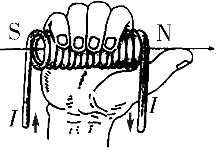
\includegraphics[width=0.98125in,height=0.68889in]{media/image337.png} &
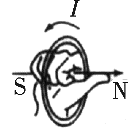
\includegraphics[width=0.63194in,height=0.61319in]{media/image338.png}\tabularnewline
\bottomrule
\end{longtable}

3.安培力的大小和方向

(1)大小

若$I\parallel B$时,\_\_F=0\_\_;若$I\perp B$时,$F=BIl$.

(2)方向

总垂直于B、I所决定的平面,即一定垂直于B和I,但B与I不一定垂直.可以用左手定则来判定:伸开左手,使大拇指跟其余四个手指\_\_垂直\_\_,并且都跟手掌在\_\_同一平面内\_\_,把手放入磁场中,让磁感线\_\_垂直穿入手心\_\_,使伸开的四指指向\_\_电流\_\_的方向,那么,\_\_拇指\_\_所指的方向就是通电导线在磁场中的受力方向.

(3)两平行通电导线间的作用

同向电流相互\_\_吸引\_\_,反向电流相互\_\_排斥\_\_.

\newpage
\subsection{安培定则的应用和磁场的叠加}

1.安培定则的应用

在运用安培定则判定直线电流和环形电流的磁场时应分清``因''和``果''.

\begin{longtable}[]{@{}m{4cm}m{4cm}m{4cm}@{}}
\toprule
 & \begin{minipage}[b]{0.30\columnwidth}\raggedright
原因(电流方向)\strut
\end{minipage} & \begin{minipage}[b]{0.30\columnwidth}\raggedright
结果(磁场方向)\strut
\end{minipage}\tabularnewline
\midrule
\endhead
直线电流的磁场 & 大拇指 & 四指\tabularnewline
环形电流的磁场 & 四指 & 大拇指\tabularnewline
\bottomrule
\end{longtable}


2.磁场的叠加

磁感应强度为矢量,合成与分解遵循平行四边形定则.

{[}例1{]}(2017·全国卷\uppercase\expandafter{\romannumeral3})如图,在磁感应强度大小为$B_0$的匀强磁场中,两长直导线P和Q垂直于纸面固定放置,两者之间的距离为l.在两导线中均通有方向垂直于纸面向里的电流I时,纸面内与两导线距离均为l的a点处的磁感应强度为零.如果让P中的电流反向、其他条件不变,则a点处磁感应强度的大小为( C )

\begin{center}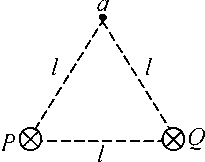
\includegraphics[width=0.93403in,height=0.73611in]{media/image339.png}\end{center}

A.0 

B.$\dfrac{\sqrt{3}}{3} B_{0}$

C.$\dfrac{2 \sqrt{3}}{3} B_{0}$ 

D.$2B_0$
\begin{solution}
	C
	
	两导线中通电流I时,两电流在a点处的磁感应强度与匀强磁场的磁感应强度的矢量合为0,则两电流磁感应强度的矢量和为$-B_0$,如图甲得$B=\dfrac{\sqrt{3}}{3} B_{0}$.P中电流反向后,如图乙,$B_{\text{合}}=B=\dfrac{\sqrt{3}}{3} B_{0}$,B合与$B_0$的矢量和为$B_{\text{总}}=\dfrac{2\sqrt{3}}{3} B_{0}$,故选项C正确.
\end{solution}

\begin{center}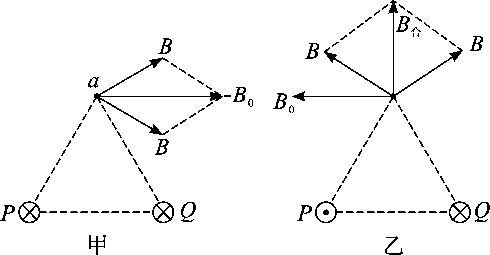
\includegraphics[width=2.22639in,height=1.16042in]{media/image340.png}\end{center}
\begin{center}
\includegraphics[width=0.70764in,height=0.12292in]{media/image13.png}\end{center}
\begin{center}
	\textbf{分析磁场的叠加的思路}
\end{center}

(1)根据安培定则确定通电导线周围磁场的方向.

(2)磁场中每一点磁感应强度的方向为该点磁感线的切线方向.

(3)磁感应强度是矢量,多个通电导体产生的磁场叠加时,合磁场的磁感应强度等于各场源单独存在时在该点磁感应强度的矢量和.

\newpage
\subsection{安培力的分析和计算}
1.计算安培力公式F=BIL,应用时要注意

(1)B与L垂直;

(2)L是有效长度

\ding{172}公式F=ILB中L指的是``有效长度''.当B与I垂直时,F最大,F=ILB;当B与I平行时,F=0.

\ding{173}弯曲导线的有效长度L,等于连接两端点线段的长度(如图所示),相应的电流沿L由始端流向末端.

\begin{center}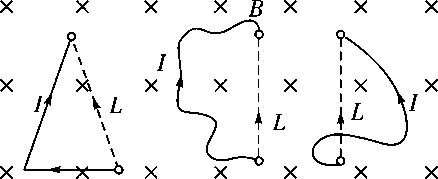
\includegraphics[width=1.99028in,height=0.81111in]{media/image341.png}\end{center}

\ding{174}闭合线圈通电后,在匀强磁场中受到的安培力的矢量和为零.

2.方向:根据左手定则判断.

{[}例2{]}(2017·全国卷Ⅰ)(多选)如图,三根相互平行的固定长直导线$L_1$、$L_2$和$L_3$两两等距,均通有电流I,$L_1$中电流方向与$L_2$中的相同,与$L_3$中的相反.下列说法正确的是( BC )

\begin{center}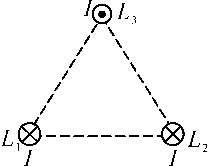
\includegraphics[width=0.94306in,height=0.75486in]{media/image342.png}\end{center}

A.$L_1$所受磁场作用力的方向与$L_2$、$L_3$所在平面垂直

B.$L_3$所受磁场作用力的方向与$L_1$、$L_2$所在平面垂直

C.$L_1$、$L_2$和$L_3$单位长度所受的磁场作用力大小之比为1:1:

D.$L_1$、$L_2$和$L_3$单位长度所受的磁场作用力大小之比为::1
\begin{solution}
	BC
	
	因三根导线中电流相等、两两等距.则由对称性可知两两之间的作用力大小均相等.因平行电流间同向吸引、反向排斥,各导线受力如图所示,由图中几何关系可知,$L_1$所受磁场作用力$F_1$的方向与$L_2$、$L_3$所在平面平行,$L_3$所受磁场作用力$F_3$的方向与$L_1$、$L_2$所在平面垂直,选项A错误,B正确.设单位长度的导线两两之间作用力的大小为F,则由几何关系可得$L_1$、$L_2$单位长度所受的磁场作用力大小为$2F\cos 60^\circ$=F,$L_3$单位长度所受的磁场作用力大小为$2F\cos 30^\circ$=F,故选项C正确,D错误.
\end{solution}

\begin{center}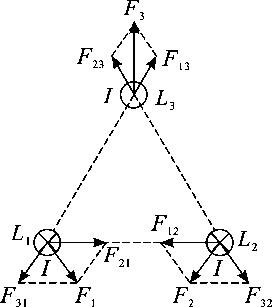
\includegraphics[width=1.23611in,height=1.39653in]{media/image343.png}\end{center}
\subsection{对安培力作用下导体运动问题的探究}

1.导体的平衡问题

通电导体在磁场中受到安培力的作用而处于平衡状态,此类问题要归结为力学问题,通过受力分析,列平衡方程求解.受力分析时,仍然遵循确定研究对象、按一定顺序分析受力的原则.需要注意的是,安培力方向的确定、安培力大小的计算要和左手定则、欧姆定律等知识相联系.

2.导线或线圈在非匀强磁场中的变速运动

此类问题中,关于安培力方向的判断是一个难点,常用的方法有:

(1)电流元法:即把整段电流等效为很多段直线电流元,先用左手定则判断出每小段电流元所受安培力的方向,从而判断出整段电流所受合力方向,最后确定运动方向.

(2)特殊值分析法:把电流或磁铁转到一个便于分析的特殊位置后再判断所受安培力方向,从而确定运动方向.

(3)等效法:环形电流可以等效成小磁针,通电螺线管可等效为很多环形电流.

(4)利用已知的一些相关结论法:\ding{172}两电流相互平行时无转动趋势,方向相同时相互吸引,方向相反时相互排斥.\ding{173}两电流不平行时有转动到平行方向相同的趋势.


\begin{center}
\includegraphics[width=0.70764in,height=0.12292in]{media/image25.png}\end{center}
\begin{center}
	\textbf{求解安培力作用下导体棒平衡问题的基本思路}
\end{center}

\begin{center}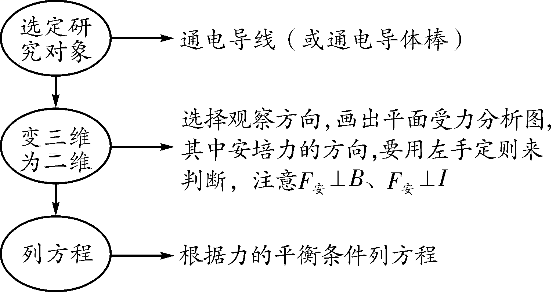
\includegraphics[width=2.52847in,height=1.32986in]{media/image345.png}\end{center}

求解关键

\ding{172}电磁问题力学化.

\ding{173}立体图形平面化.

\ding{174}求解极值数学化.

\newpage
\section{磁场对运动电荷的作用}

1.洛伦兹力的大小和方向

(1)定义:磁场对\_\_运动电荷\_\_的作用力.

(2)大小

\ding{172}$v\parallel B$时,F=0;

\ding{173}$v\perp B$时,F=qvB;

\ding{174}v与B夹角为$\theta$时,$F=qvB\sin \theta$.

(3)方向

\ding{172}判定方法:应用左手定则,注意四指应指向正电荷运动方向或负电荷运动的反方向;

\ding{173}方向特点:F$\perp$B,F$\perp$v.即F垂直于B、v决定的平面.(注意B和v可以有任意夹角)

2.带电粒子在匀强磁场中的运动

(1)若$v\parallel B$,带电粒子以入射速度v做\_\_匀速直线\_\_运动.

(2)若$v\perp B$,带电粒子在垂直于磁感线的平面内,以入射速度v做\_\_匀速圆周\_\_运动.

(3)基本公式

\ding{172}向心力公式:$q v B=m \dfrac{v^{2}}{r}$;

\ding{173}轨道半径公式:$r=-\dfrac{m v}{B q}$;

\ding{174}周期公式:$T=\dfrac{2 \pi m}{q B}$.
\newpage
\subsection{对洛伦兹力的理解}

1.洛伦兹力的特点

(1)利用左手定则判断洛伦兹力的方向,注意区分正、负电荷.

(2)当电荷运动方向发生变化时,洛伦兹力的方向也随之变化.

(3)运动电荷在磁场中不一定受洛伦兹力作用.

(4)洛伦兹力一定不做功.

2.洛伦兹力与电场力的比较

\begin{longtable}[]{@{}m{4cm}m{4cm}m{4cm}@{}}
\toprule
& 洛伦兹力 & 电场力\tabularnewline
\midrule
\endhead
产生条件 & $v\neq 0$且v不与B平行 & 电荷处在电场中\tabularnewline
大小 & F=qvB(v$\perp$B) & F=qE\tabularnewline

力方向与场方向的关系
& \begin{minipage}[t]{0.30\columnwidth}\raggedright
F$\perp$B,F$\perp$v\strut
\end{minipage} & \begin{minipage}[t]{0.30\columnwidth}\raggedright
F$\parallel$E\strut
\end{minipage}\tabularnewline
做功情况 & 任何情况下都不做功 & 可能做功,也可能不做功\tabularnewline
\bottomrule
\end{longtable}

\begin{center}
\includegraphics[width=0.70764in,height=0.12292in]{media/image13.png}\end{center}
\begin{center}
	\textbf{洛伦兹力与安培力的联系及区别}
\end{center}


(1)安培力是洛伦兹力的宏观表现,二者是相同性质的力,都是磁场力.

(2)安培力可以做功,而洛伦兹力对运动电荷不做功.
\newpage
\subsection{带电粒子在匀强磁场中的运动}

1.圆心的确定

(1)基本思路:与速度方向垂直的直线和图中弦的中垂线一定过圆心.

(2)两种常见情形

\ding{172}已知入射方向和出射方向时,可通过入射点和出射点分别作垂直于入射方向和出射方向的直线,两条直线的交点就是圆弧轨道的圆心(如图甲所示,图中P为入射点,M为出射点)

\begin{center}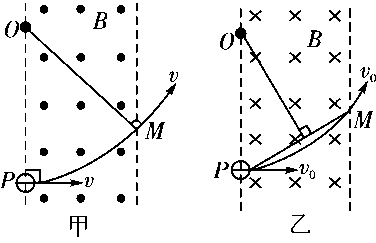
\includegraphics[width=1.70764in,height=1.10347in]{media/image353.png}\end{center}

\ding{173}已知入射点和出射点的位置时,可以先通过入射点作入射方向的垂线,再连接入射点和出射点,作其中垂线,这两条垂线的交点就是圆弧轨道的圆心.(如图乙所示,图中P为入射点,M为出射点)

2.半径的确定和计算

利用平面几何关系,求出该圆的可能半径(或圆心角),并注意以下两个重要的几何特点:

(1)粒子速度的偏向角$\varphi$等于圆心角$\alpha$,并等于AB弦与切线的夹角(弦切角$\theta$)的2倍(如图所示),即$\varphi=\alpha=2\theta=\omega t$.

\begin{center}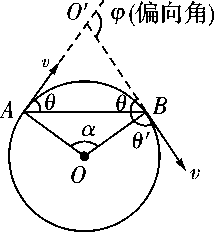
\includegraphics[width=0.97153in,height=1.05694in]{media/image354.png}\end{center}

(2)相对的弦切角$\theta$相等,与相邻的弦切角$\theta^\prime$互补,即两角之和$\theta+\theta^\prime=180^\circ$.

3.运动时间的确定

粒子在磁场中运动一周的时间为T,当粒子运动的圆弧所对应的圆心角为$\alpha$时,其运动时间由下式表示:

$t=\dfrac{\alpha}{360^{\circ}} T\left(\text { 或 } t=\dfrac{\alpha}{2 \pi} T\right)$.

\begin{center}
\includegraphics[width=0.70764in,height=0.12292in]{media/image25.png}\end{center}
\begin{center}
	\textbf{带电粒子在磁场中做匀速圆周运动的解题步骤}
\end{center}

\begin{center}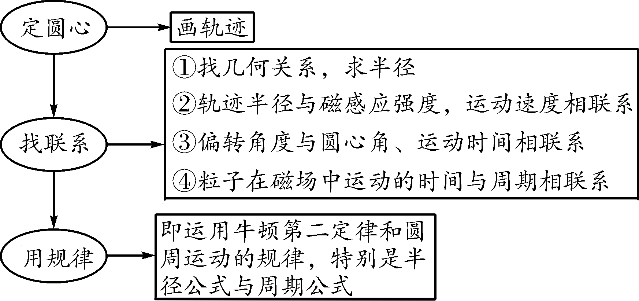
\includegraphics[width=2.90556in,height=1.36806in]{media/image355.png}\end{center}

\subsection{带电粒子在磁场中运动的多解问题}

\begin{center}
\includegraphics[width=0.70764in,height=0.12292in]{media/image13.png}\end{center}
\begin{center}
	\textbf{求解带电粒子在磁场中运动多解问题的技巧}
\end{center}

(1)分析题目特点,确定题目多解的形成原因.

(2)作出粒子的运动轨迹示意图(全面考虑多种可能性).

(3)若为周期性重复的多解问题,寻找通项式,若是出现几种解的可能性,注意每种解出现的条件.

1.带电粒子电性不确定形成多解

受洛伦兹力作用的带电粒子,可能带正电,也可能带负电,在相同的初速度的条件下,正、负粒子在磁场中运动轨迹不同,形成多解.

如图,带电粒子以速率v垂直进入匀强磁场,如带正电,其轨迹为a,如带负电,其轨迹为b.

\begin{center}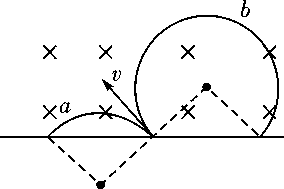
\includegraphics[width=1.29236in,height=0.85833in]{media/image358.png}\end{center}


2.磁场方向不确定形成多解

有些题目只告诉了磁感应强度的大小,而未具体指出磁感应强度方向,此时必须要考虑磁感应强度方向不确定而形成的多解.


3.临界状态不唯一形成多解

带电粒子在洛伦兹力作用下飞越有界磁场时,由于粒子运动轨迹是圆弧状,因此,它可能穿过去了,也可能转过180°从入射界面这边反向飞出,于是形成了多解,如图所示.

\begin{center}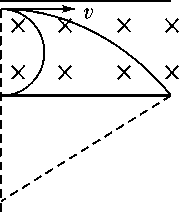
\includegraphics[width=0.81111in,height=0.9625in]{media/image360.png}\end{center}


4.运动的周期性形成多解

带电粒子在部分是电场,部分是磁场的空间运动时,运动往往具有往复性,从而形成多解,如图所示.

\begin{center}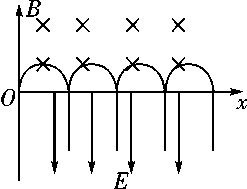
\includegraphics[width=1.12292in,height=0.85833in]{media/image362.png}\end{center}
\newpage
\section{带电粒子在复合场中的运动}

1.带电粒子在复合场中的运动

(1)复合场与组合场

\ding{172}复合场:电场、磁场、重力场共存,或其中某两场共存.

\ding{173}组合场:电场与磁场各位于一定的区域内,并不重叠,或在同一区域,电场、磁场分时间段或分区域交替出现.

(2)三种场的比较

\begin{longtable}[]{@{}m{1cm}m{6cm}m{5cm}@{}}
\toprule
 & \begin{minipage}[b]{0.30\columnwidth}\raggedright
力的特点\strut
\end{minipage} & \begin{minipage}[b]{0.30\columnwidth}\raggedright
功和能的特点\strut
\end{minipage}\tabularnewline
\midrule
\endhead
\begin{minipage}[t]{0.30\columnwidth}\raggedright
重力场\strut
\end{minipage} & \begin{minipage}[t]{0.30\columnwidth}\raggedright
大小:G=mg

方向:竖直向下\strut
\end{minipage} & \begin{minipage}[t]{0.50\columnwidth}\raggedright
重力做功与路径无关

重力做功改变物体的重力势能\strut
\end{minipage}\tabularnewline
\begin{minipage}[t]{0.30\columnwidth}\raggedright
静电场\strut
\end{minipage} & \begin{minipage}[t]{0.50\columnwidth}\raggedright
大小:F=qE

方向:a.正电荷受力方向与场强方向相同

b.负电荷受力方向与场强方向相反\strut
\end{minipage} & \begin{minipage}[t]{0.30\columnwidth}\raggedright
电场力做功与路径无关

W=qU

电场力做功改变电势能\strut
\end{minipage}\tabularnewline
\begin{minipage}[t]{0.30\columnwidth}\raggedright
磁场\strut
\end{minipage} & \begin{minipage}[t]{0.30\columnwidth}\raggedright
洛伦兹力F=qvB

方向符合左手定则\strut
\end{minipage} & \begin{minipage}[t]{0.30\columnwidth}\raggedright
洛伦兹力不做功,不改变带电粒子的动能\strut
\end{minipage}\tabularnewline
\bottomrule
\end{longtable}

(3)带电粒子在复合场中的运动分类

\ding{172}静止或匀速直线运动

当带电粒子在复合场中所受合外力为零时,将处于静止状态或做\_\_匀速直线运动\_\_.

\ding{173}匀速圆周运动

当带电粒子所受的重力与电场力大小\_\_相等\_\_,方向\_\_相反\_\_时,带电粒子在洛伦兹力的作用下,在垂直于匀强磁场的平面内做\_\_匀速圆周\_\_运动.

\ding{174}较复杂的曲线运动

当带电粒子所受合外力的大小和方向均变化,且与初速度方向不在同一条直线上时,粒子做\_\_非匀\_\_变速曲线运动,这时粒子运动轨迹既不是圆弧,也不是抛物线.

\ding{175}分阶段运动

带电粒子可能依次通过几个情况不同的复合场区域,其运动情况随区域发生变化,其运动过程由几种不同的运动阶段组成.
\newpage
2.电场、磁场分区域应用实例

\begin{center}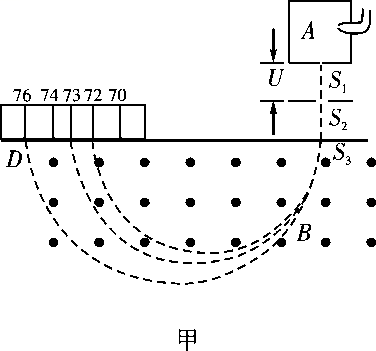
\includegraphics[width=1.70764in,height=1.59444in]{media/image369.png}\end{center}

(1)质谱仪

\ding{172}构造:如图甲所示,由粒子源、加速电场、偏转磁场和照相底片等构成.

\ding{173}原理:粒子由静止被加速电场加速,根据动能定理可得关系式$q U=\dfrac{1}{2} m v^{2}$.

粒子在磁场中受洛伦兹力作用而偏转,做匀速圆周运动,

根据牛顿第二定律得关系式$q v B=m \dfrac{v^{2}}{r}$.

由两式可得出需要研究的物理量,如粒子轨道半径、粒子质量、比荷.

$r=\dfrac{1}{B} \sqrt{\dfrac{2 m U}{q}}-m=\dfrac{q r^{2} B^{2}}{2 U}-\dfrac{q}{m}=-\dfrac{2 U}{B^{2} r^{2}}$.

(2)回旋加速器

\begin{center}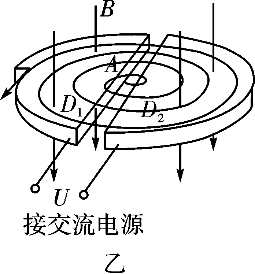
\includegraphics[width=1.49028in,height=1.59931in]{media/image370.png}\end{center}

\ding{172}构造:如图乙所示,$D_1$、$D_2$是半圆形金属盒,D形盒的缝隙处接交流电源,D形盒处于匀强磁场中.

\ding{173}原理:交流电的周期和粒子做圆周运动的周期相等,粒子在圆周运动的过程中一次一次地经过D形盒缝隙,两盒间的电势差一次一次地反向,粒子就会被一次一次地加速.由$q v B=m \dfrac{v^{2}}{r}$,得$E_{\mathrm{km}}=\dfrac{q^{2} B^{2} r^{2}}{2 m}$,可见粒子获得的最大动能由磁感应强度B和D形盒半径r决定,与加速电压无关.
\newpage
3.电场、磁场同区域并存的实例

\begin{longtable}[]{@{}m{2.2cm}m{3cm}m{6cm}@{}}
\toprule
装置 & 原理图 & 规  律\tabularnewline
\midrule
\endhead

速度
选择器
&
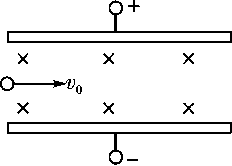
\includegraphics[width=1.05694in,height=0.75486in]{media/image371.png}
&
若$q v_{0} B=q E$,即$v_{0}=\dfrac{E}{B}$,粒子做匀速直线运动
\tabularnewline

磁流体
发电机
&
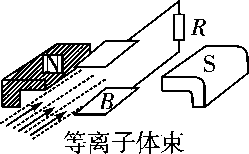
\includegraphics[width=1.13194in,height=0.69792in]{media/image372.png}
&
等离子体射入,受洛伦兹力偏转,使两极板带电,当$q \dfrac{U}{d}=q v_{0} B$时,两极板间能达到最大电势差$U=Bv_0d$
\tabularnewline
电磁
流量计
&
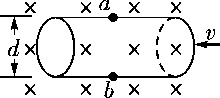
\includegraphics[width=1in,height=0.44306in]{media/image373.png}
&
当 $q \dfrac{U}{d}=q v B$ 时,有 $v=-\dfrac{U}{B d} \quad,$ 流量 $Q=S v=\dfrac{\pi d U}{4 B}$
\tabularnewline
霍尔
效应
&
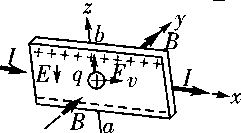
\includegraphics[width=1.09444in,height=0.60347in]{media/image374.png}
&
在匀强磁场中放置一个矩形截面的载流导体,当磁场方向与电流方向垂直时,导体在与磁场、电流方向都垂直的方向上出现了电势差,这种现象称为霍尔效应
\tabularnewline
\bottomrule
\end{longtable}
\newpage
\subsection{带电粒子在组合场中的运动问题}
带电粒子在组合场中的运动问题为高考热点,考查学生对带电粒子在先后出现(或交替出现)的电磁场中的运动分析、性质判断及综合计算能力.

1.是否考虑粒子重力的三种情况

(1)对于微观粒子,如电子、质子、离子等,因为其重力一般情况下与电场力或磁场力相比太小,可以忽略,而对于一些宏观物体,如带电小球、液滴、金属块等一般应当考虑其重力.

(2)在题目中有明确说明是否要考虑重力的,这种情况比较正规,也比较简单.

(3)不能直接判断是否要考虑重力的,在进行受力分析与运动分析时,要由分析结果确定是否要考虑重力.

2.带电粒子在组合场中运动,要分段处理,对匀强电场中的匀变速直线运动或类平抛运动,可由牛顿定律及运动学公式求解,对匀强磁场中的匀速圆周运动,要结合几何知识,确定圆心及半径,从而确定磁感应强度和圆心角或时间,确定从电场进入磁场的速度的大小、方向及两场交界处轨迹的几何关系,是解决问题的关键.

\begin{center}
\includegraphics[width=0.70764in,height=0.12292in]{media/image25.png}\end{center}
\begin{center}
	\textbf{解决带电粒子在组合场中运动问题的思路方法}
\end{center}

\begin{center}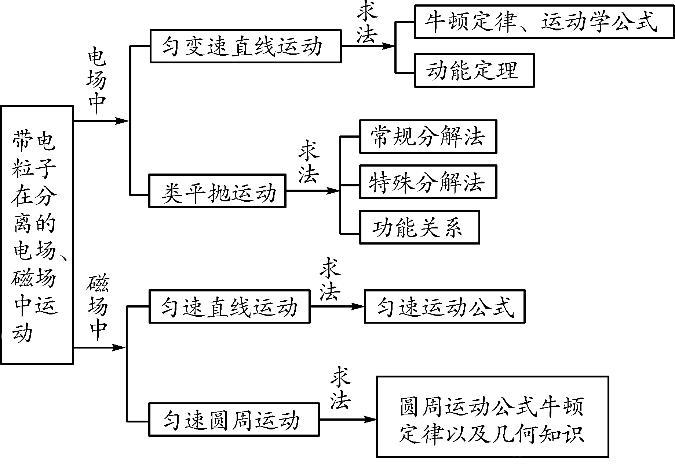
\includegraphics[width=3.06597in,height=2.15069in]{media/image377.png}\end{center}

{[}例1{]}(2017·天津卷)平面直角坐标系xOy中,第Ⅰ象限存在垂直于平面向里的匀强磁场,第\uppercase\expandafter{\romannumeral3}象限存在沿y轴负方向的匀强电场,如图所示.一带负电的粒子从电场中的Q点以速度$v_0$沿x轴正方向开始运动,Q点到y轴的距离为到x轴距离的2倍.粒子从坐标原点O离开电场进入磁场,最终从x轴上的P点射出磁场,P点到y轴距离与Q点到y轴距离相等.不计粒子重力,问:

\begin{center}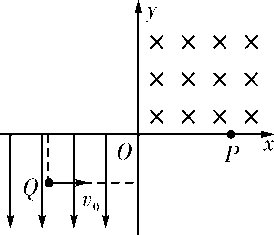
\includegraphics[width=1.24514in,height=1.06597in]{media/image378.png}\end{center}

(1)粒子到达O点时速度的大小和方向;

(2)电场强度和磁感应强度的大小之比.
\begin{solution}
	(1)$\sqrt{2} v_0$ 速度方向与x轴正方向成$45^\circ$角斜向上

(2)$\dfrac{v_0}{2}$
\end{solution} 

\subsection{带电粒子在复合场中的运动问题}

带电粒子在复合场中的运动问题是历年高考命题的热点,覆盖面大,综合性强,难度大,能力要求高,以计算题呈现,有时也有选择题.

1.带电粒子在复合场中无约束情况下的运动主要是以下几种形式

\begin{longtable}[]{@{}m{4cm}m{9cm}@{}}
\toprule
复合场组成 & 可能的运动形式\tabularnewline
\midrule
\endhead
\begin{minipage}[t]{1\columnwidth}\raggedright
磁场、重力场并存\strut
\end{minipage} & \begin{minipage}[t]{0.9\columnwidth}\raggedright
\ding{172}若重力和洛伦兹力平衡,则带电体做匀速直线运动

\ding{173}若重力和洛伦兹力不平衡,则带电体将做复杂的曲线运动,

因F洛不做功,故机械能守恒,由此可求解问题\strut
\end{minipage}\tabularnewline
\begin{minipage}[t]{0.47\columnwidth}\raggedright
电场、磁场并存

(不计微观粒子的重力)\strut
\end{minipage} & \begin{minipage}[t]{0.9\columnwidth}\raggedright
\ding{172}若电场力和洛伦兹力平衡,则带电体做匀速直线运动

\ding{173}若电场力和洛伦兹力不平衡,则带电体做复杂的曲线运动,

因F洛不做功,可用动能定理求解问题\strut
\end{minipage}\tabularnewline
\begin{minipage}[t]{0.47\columnwidth}\raggedright
电场、磁场、重力场并存\strut
\end{minipage} & \begin{minipage}[t]{0.9\columnwidth}\raggedright
\ding{172}若三力平衡,带电体一定做匀速直线运动

\ding{173}若重力与电场力平衡,带电体一定做匀速圆周运动

\ding{174}若合力不为零且与速度方向不垂直,带电体将做复杂的曲线运动,

因F洛不做功,可用能量守恒定律或动能定理求解问题\strut
\end{minipage}\tabularnewline
\bottomrule
\end{longtable}

2.分阶段运动

带电粒子可能依次通过几个情况不同的复合场区域,其受力情况随区域发生变化,则其运动过程由几种不同的运动阶段组成.


